\documentclass{ctexart}

\usepackage{amsmath}
\usepackage{amssymb}
\usepackage{graphicx}

\begin{document}

本章介绍经典的序列决策形式化模型——有限MDP,它既像bandit一样涉及评估性回馈,也包含结合性回馈——在不同的形势中选择不同行动。因为能做出精确的理论描述,因此MDP是强化学习问题的理想数学形式。

\section{代理环境接口}

MDP试图直接构造从互动中学习以实现某一目标的问题。学习者或决策者称为\text{代理(agent)},与它互动的代理外一切事物为\textbf{环境(enviroment)}。它们在离散的时间步$t=0,1,2,\dots$上互动,在每一步$t$,代理处在环境的某个\textbf{状态(state)}$S_t \in \mathcal S$中,基于此选择一个\textbf{行动(action)}$A_t \in \mathcal A(s)$,一步之后,代理获得一个数值\textbf{激励(reward)}$R_{t+1} \in \mathcal R \in \mathbb R$,并进入新的状态$S_{t+1}$。如下图:
\begin{figure}[htbp]
    \centering
    
\includegraphics[width = 1.\linewidth]{/Users/tesla/Articles/rl.trans/figures/0301.png}
    \caption{代理-环境接口}
    \label{fig:0301} 
\end{figure}
其中$\mathcal A(s)$表示在状态$s$代理可选的行动集;因此这就产生了这样一个\textbf{序列(sequence)}或\textbf{轨迹(trajectory)}:
\begin{equation}
    S_0,A_0,R_1,S_1,A_1,R_2,S_2,A_2,R_3,\dots
\end{equation}
在有限MDP中,状态集$\mathcal S$、行动集$\mathcal A$和激励集$\mathcal R$都是有限的,这样随机变量$R_t$和$S_t$都有良好定义、仅依赖前个状态-行动对的离散概率分布,即对所有的$s',s \in \mathcal S$,$r \in \mathcal R$和$a \in \mathcal A(s)$有:
\begin{equation}
    p(s',r\mid s,a) \dot= \text{Pr}\{S_{t+1}=s',R_{t+1}=r \mid S_t=s,A_t=a \}
\end{equation}
等号上的点表示这个公式是一个定义,函数$p:\mathcal{S \times R \times S \times A} \to [0,1]$是一个4-参数的随机性函数,为每个状态-行动对$s,a$确定了概率分布:
\begin{equation}
    \sum_{s'\in\mathcal S}\sum_{r\in\mathcal R}p(s',r \mid s,a) = 1, \qquad \forall s\in\mathcal S,a\in\mathcal A(s)
\end{equation}
由4-参数函数$p$给出的概率完全刻划了一个有限MDP的\textbf{动态(dynamics)},由此能计算出关于环境的一切。要注意是代理-环境边界与通常的物理边界不同,通常原则是任意无法被代理随意改变的内容都属于环境,即表示代理的绝对控制而非认知边界,也会因不同的原因放置在不同的地方。

\section{激励和回报}

代理的目标是最大化激励获得的总激励,这样用激励来形式化目标的思想是RL的最独特性质,并且已在实践中证明了足够的灵活性和广泛的可用性。激励信号是告诉代理什么是要达到的,而非如何达到。任务可分为2种:
\begin{itemize}
    \item 一种是有明显的终止状态、可将交互自然切分子序列的分节任务;
    \item 另一种则是一直持续永无极限的连续任务;
\end{itemize}
回报是激励序列的特定函数,在所有任务中可统一定义为:
\begin{align}
    G_t &\dot= R_{t+1} + \gamma R_{t+2} + \gamma^2 R_{t+3} + \cdots = \sum_{k=0}^T \gamma^k R_{t+k+1} \\
        &= R_{t+1} + \gamma\left( \sum_{k=1}^T\gamma^kR_{t+k+1} \right) \notag \\
        &= R_{t+1} + \gamma G_{t+1}
\end{align}
其中$\gamma \in [0,1]$是折扣因子,表示未来激励的当前价值:$k$步之后获得的激励仅是当前同样值的$\gamma^{k-1}$倍。

\section{策略和价值函数}

RL中策略是从状态到选择每个可能行动的概率,$\pi(a\mid s)$是中的"|"仅表示它为每个$s \in \mathcal S$在$a \in \mathcal A(s)$上定义的概率分布。一个状态$s$在策略$\pi$下的\textbf{价值},记为$v_\pi(s)$,为从状$s$开始遵循$\pi$所能获得的期望回报:
\begin{align}
    v_\pi(s) &\dot= \mathbb E_\pi[G_t\mid S_t=s] \\
             &= \sum_a\pi(a\mid s)\sum_{s',r} p(s',r\mid s,a)\bigl[ r+\gamma v_\pi(s') \bigr] \qquad \forall s \in \mathcal S
\end{align}
函数$v_\pi$是策略$\pi$的状态价值函数。(3.7)为$v_\pi$的贝尔曼(Bellman)方程(证明见附录),表达了状态与其后继状态之间的价值关系,这种关系也可以由下图来表现:
\begin{figure}[htbp]
    \centering
    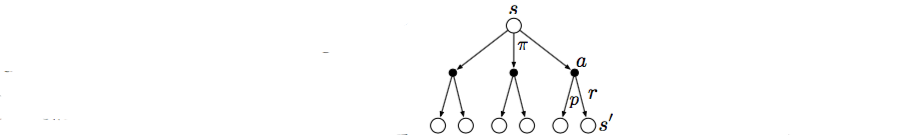
\includegraphics[width = 1.\linewidth]{/Users/tesla/Articles/rl.trans/figures/0302.png}
    \caption{备份图}
    \label{fig:0302} 
\end{figure}
上图称为$v_\pi$的备份图,因其勾勒形成更新基础的关系,或备份RL方法中的核心操作——将价值信息从后继状态反向传播。同样可定义状态-行动对的价值:
\begin{align}
    q_\pi(s,a) &\dot= \mathbb E_\pi\left[ G_t\mid S_t=s, A_t=a \right] \\
               &= \sum_{s',r} p(s',r\mid s,a) \left[ r+\gamma\sum_{a'}\pi(a'\mid s') q_\pi(s',a') \right]
\end{align}
其中$q_\pi$是策略$\pi$的行动价值函数。(3.9)为$q_\pi$的贝尔曼(Bellman)方程,$q_\pi$的备份图为:
\begin{figure}[htbp]
    \centering
    
\includegraphics[width = 1.\linewidth]{/Users/tesla/Articles/rl.trans/figures/0303.png}
    \caption{备份图}
    \label{fig:0303} 
\end{figure}
状态价值函数和行动价值函数的关系:
\begin{align}
    v_\pi(s) &= \sum_a \pi(a\mid s)q_\pi(s,a) \tag{3.10}\\
    q_\pi(s,a) &= \sum_{s',r} p(s',r \mid s,a)[r+\gamma v_\pi(s')] \tag{3.11}
\end{align}
需要声明的一点是:价值函数是贝尔曼方程的唯一解。

\section{最优策略与最优价值函数}

定义策略的偏序关系为,当且仅当对所有的$s\in\mathcal S$都有$v_\pi(s)\ge v_{\pi'}(s)$时,则$\pi\ge\pi'$;总存在一个或多个策略优于或等于其他所有策略,此即最优策略记为$\pi_*$;所有最优策略都有同样的最优状态价值函数$v_*(s)\dot=\max_\pi v_\pi(s)$;所有最优策略都有同样的最优行动价值函数,表示在状态$s$采取行动$a$后遵循最优策略所能得到的期望回报:
\begin{align}
    q_*(s,a) &\dot= \max_\pi q_\pi(s,a)\notag \\
             &= \max_\pi \mathbb E_\pi\bigl[ G_t \mid S_t=s, A_t=a \bigr]\notag \\
             &= \max_\pi\mathbb E_\pi\bigl[ R_{t+1} + \gamma G_{t+1} \mid S_t=s, A_t=a \bigr]\notag \\
             &= \max_\pi \mathbb E_\pi\bigl[ R_{t+1} + \gamma G_{t+1} \mid S_{t+1}, S_t=s,A_t=a \bigr] \\
             &= \mathbb E\bigl[ R_{t+1}+\gamma v_*(S_{t+1}) \mid S_t=s,A_t=a \bigr]
\end{align}
(3.12)是因为条件为$S_t=s,A_t=a$时就可以引出后继状态$S_{t+1}$;还有这里形式是$\mathbb[G_{t+1}\mid S_t=s,A_t=a]$,回报与状态行动不在同一时间步,因此不是$q(s,a)$。注意这里是采取行动$a$后再遵循最优策略,在状态$s$采取行动$a$很可能并不属于最优策略。

因$v_*$是策略的价值函数,并且是最优的,因此满足\textbf{贝尔曼最优性方程}:
\begin{align}
    v_*(s)
    &= \max_{a\in\mathcal A(s)} q_{\pi_*}(s,a)\notag \\
    &= \max_a \mathbb E_{\pi_*}[G_t \mid S_t=s, A_t=a]\notag \\
    &= \max_a \mathbb E_{\pi_*}[R_{t+1} + \gamma G_{t+1} \mid S_t=s, A_t=a] \\
    &= \max_a \mathbb E_{\pi_*}[R_{t+1} + \gamma v_*(S_{t+1}) \mid S_t=s, A_t=a] \\
    &= \max_a \sum_{s',r} p(s',r \mid s,a)\bigl[r+\gamma v_*(s')\bigr]
\end{align}
最后两个公式为两种形式的贝尔曼最优性方程。$q_*$的贝尔曼最有性方程为:
\begin{align}
    q_*(s,a)
    &= \mathbb E\left[ R_{t+1}+\gamma\max_{a'}q_*(S_{t+1}, a') \middle| S_t=s, A_t=a \right]\notag \\
    &= \sum_{s',r}p(s',r\mid s,a)\left[ r+\gamma\max_{a'}q_*(s',a') \right] 
\end{align}
$v_*,q_*$的贝尔曼最有性方程的备份图如下,这里用最大取代了前面$v_\pi,q_\pi$备份图中的期望:
\begin{figure}[htbp]
    \centering
    
\includegraphics[width = 1.\linewidth]{/Users/tesla/Articles/rl.trans/figures/0304.png}
    \caption{备份图}
    \label{fig:0304} 
\end{figure}

对有限MDP,$v_\pi$的贝尔曼最优性方程含有与策略无关的唯一解。贝尔曼方程实际是一个方程组,每个方程对应一个状态。若有$n$个状态,则有$n$个方程含$n$个未知数。若环境动态$p$已知,则原则上可以解出这个$v_*$的方程组。类似也可以$q_*$相关的方程组。

获得$v_*$后,仅对每个状态$s$获得最大价值的行动赋予非零值的策略就是最优策略,即任意关于$v_*$贪心的策略即为最优;因$v_*$\textbf{已考虑所有可能未来行为的激励结果},其对短期后果贪心的策略实际就是长期的;获得$q_*$后,找到使$q_*(s,a)$最大的行动即可获得最优策略,甚至无需知道任何环境动态的信息。

显然贝尔曼最优性方程提供了活的最优策略的一种途径,但依赖至少三个实际中很少成立的假设:1)确切知道环境的动态信息;2)充足的计算资源;3)马尔科夫特性。RL通常只能诉诸近似方法。

许多方法可以视为近似解决贝尔曼最优性方程的方法。比如启发式搜索(Heuristic Search, HS)可视为将(3.15)的右侧扩展几次到某个深度,形成一棵概率“树”,然后在“页”节点使用启发式方法近似$v_*$;动态规划则更接近贝尔曼最优性方程。许多强化学习方法都可以清晰地理解为使用实际经历的转移代替期望转移的知识来近似解决贝尔曼方程。

\end{document}
